\documentclass{article}

\usepackage[letterpaper]{geometry}
\usepackage{graphicx}

\graphicspath{{./img/}}

\title{2411 Project 6}
\author{Duncan Wilkie}
\date{12 November 2021}

\begin{document}

\maketitle

\section{Analytical Solution}
It is expected that a simple stochastic process like this will have radial displacement at step $i$ of $\overline{\Delta r}\sqrt{i}$.

\section{Numerical Method}
We use the Linux \verb{drand48()} fuction seeded with the value 42 to compute the step for a walk of length 1000, implemented in C++.

\section{Program Analysis}
The program written appears in the script files. The resulting plot of the random walk appears below, showing precisely the standard Brownian motion qualitative behavior. 
\[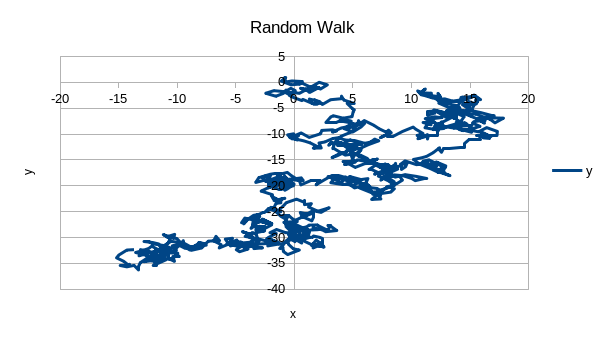
\includegraphics[scale=0.5]{plot1.png}\]
A plot of the real displacement versus the expected value appears below. It is evident it is followed approximately, but that the deviations from it can become rather high.

\[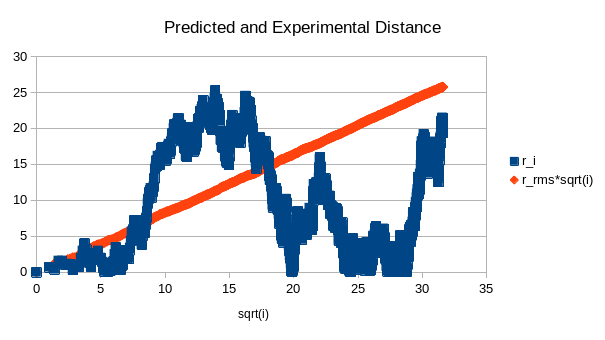
\includegraphics[scale=0.5]{plot2.png}\]
After the program has completed, the average displacement is $0.815$ meters on each step. This corresponds to an approximate total distance travelled of $r_{rms}N=815$ meters. The actual distance away from the origin, on the other hand, is 19 meters. The first is clearly much larger, and so this is clearly not a terribly efficient form of travel.

\section{Script Files}
\end{document}
%%% Local Variables:
%%% mode: latex
%%% TeX-master: t
%%% End:
